
%use mybib.bib for bibliography. bibtex is used for bibliography
\documentclass[journal]{IEEEtran}
\usepackage[utf8]{inputenc}
\usepackage{graphicx}
\usepackage{cite}
\usepackage{longtable}
\usepackage{amsmath}
\usepackage{multirow}
\usepackage{multicol}
%\usepackage{wrapfig}
\usepackage{float}
%\usepackage[section]{placeins}
%\usepackage{subcaption}
\usepackage{array}
\usepackage[export]{adjustbox}
\usepackage{tabu}
\usepackage{tabularx}
\usepackage{listings}
\usepackage{siunitx}
\usepackage{siunitx}
\usepackage{ wasysym }
\usepackage[usenames, dvipsnames]{color}


%%%%%%%%%%%%%%%%%%%%%%%%%%%%%%%%%%%%%%%%%%%%%%%%%%%%%


\ifCLASSINFOpdf

\else

\fi


\hyphenation{op-tical net-works semi-conduc-tor}


\begin{document}

\title{A Graph Search Based Optimal Control Technique for Enterprise Level Energy Storage Based on Forecasting of PV, Load and Real-Time price of Energy}

\author{ Alvi~Newaz,~\IEEEmembership{Student Member,~IEEE,}
Juan~Ospina,~\IEEEmembership{Student Member,~IEEE and}
     M.~Omar~Faruque,~\IEEEmembership{Senior Member,~IEEE}
        }% <-this % stops a space





\maketitle                                                               

\begin{abstract}
This paper proposes a novel energy storage management (ESM) solution designed to optimize the use of grid-connected distributed energy resources (DERs) based on forecasting of generation, load, and real-time energy prices. The proposed control strategy aims to control the operations of the energy storage (ES) so that the total cost of energy used to serve the local electrical load is minimized. The proposed solution uses the energy storage status and available data to generate a graph that is explored using the A* search algorithm with the objective of finding the optimum cost of energy. Seven-day offline test results are presented for two different scenarios. The first scenario compares the A* based ESM with two base test cases considering net metering. The other scenario compares the A* based ESM with the same base test cases considering different costs for buying power from the grid and selling power to the grid. Two-day real-time simulation results are also presented considering different costs for buying power from the grid and selling power to the grid. The pricing schemes used in the testing were obtained from the Pacific Gas and Electric (PG\&E) and the New York Independent System Operator (NYISO). The results show substantial cost savings over the compared schemes. %\textbf{MAYBE, ADD THE \% OF COST SAVINGS OR THE BEST ONES}
\end{abstract}


\begin{IEEEkeywords}
 A* Search Algorithm, Distributed Energy Resources, Energy Storage Management, Energy Storage System, Graph Search, Real-Time Pricing, Real-Time Simulation.
\end{IEEEkeywords}

\IEEEpeerreviewmaketitle


\section{Introduction}
In the last few years, there has been significant growth in grid-connected distributed energy resources (DERs) leading to an increased deployment of distributed generation (DG) and recently more distributed storage (DS) systems. Companies are starting to heavily invest in the competitive energy storage system market by taking advantage of the decreasing costs of energy storage. Although a significant amount of DG and DS are being added to the distribution grid, need to improve their control systems for seamless integration to the grid is still there. In the US, most DG and DS systems are deployed to either help reduce the metered load through net-metering programs or to sell power to the utility through power purchase agreements (PPAs). The potential of DG combined with DS is not fully utilized under these pricing schemes due to the lack of proper control. in order to maximize the use of available DERs, a state-of-the-art energy management solution is a necessity for our future electrical grid . Such an energy management solution will be able to dynamically optimize the use of all the available DS with the objective of serving the load in the most economical and safe way possible. This will benefit both utility companies and regular consumers. Due to the constraints and intermittent nature of some DG systems, such as wind and solar, the optimum management of DS combined with a DG is a difficult problem to solve. The most common approaches found in the current literature are as follows. Some researchers formulate the problem as a linear programming (LP) or mixed integer linear programming (MILP) model \cite{lp73, lp74, lp75}. Authors in \cite{pso80, pso81} present an energy management solution based on particle swarm optimization for a microgrid containing wind turbines and energy storage (ES) system. Other researchers propose crow-search and ant colony optimization models to solve the energy management problem for local microgrids as seen in \cite{csa87} and \cite{aco84}. There have also been model predictive control (MPC) based approaches for managing ES in microgrid settings as seen in \cite{energymanajaboulay,mpcmorstyn}.  Researchers in \cite{ga76, ga77} have also proposed genetic algorithm based solutions to optimize the ES operation in a microgrid. One clear disadvantage of these proposed models is that most of these approaches only consider the current status of the system and ignore some critical factors like energy tariff, forecasted load, and forecasted generation profiles.  These information can be used to find an optimum solution based on both current and probable future states of the system as opposed to a solution relying only on the currently available data. Off-line day ahead planning models have also been proposed in the literature. In these methods, available predicted data is used to optimize the scheduling of the ES based on Monte Carlo simulations \cite{6872821,7010943,6839110}. These solutions are very computationally intensive and require a lot of time for planning the day ahead. The computational complexity makes them unsuitable for real-time implementation. Also, as they are off-line calculations they rely vastly on the accuracy of the predictions.

From the discussion thus far, it is evident that there is a need for a real-time ESM solution that can optimize the long-term operating costs of a system containing DG and an energy storage (ES) system. This paper presents an optimum real-time control strategy for such systems. The proposed control strategy takes into account the present and forecasted states of the system, together with the real-time price (RTP), in order to optimize the cost of energy usage. The rest of the paper is organized as follows. Section II discusses how the ESM problem is formulated as a graph search problem. Section III introduces the A* graph search algorithm used to find the optimal solution and how it is used to search for the optimum path of energy decisions. Section IV discusses the test system used in simulation to validate the performance of the graph search based ESM algorithm. Section V discusses the results obtained from the offline simulation and section VI presents the real-time simulation results. Section VII talks about the novelty of the research and section VIII presents the conclusions.

\section{Problem formulation} \label{formulation}
The proposed solution technique is designed to be implemented at the point of common coupling (PCC) of a microgrid containing distributed generation (DG) and energy storage (ES). Fig. \ref{fig:system_arch} depicts an example system. Here, the energy storage management system (ESMS) is in charge of controlling the battery connected to the grid with the objective of getting the most cost optimum use of the resources available. The objective of the ESMS is to optimize the use cost of energy storage under different pricing schemes by taking advantage of RTP or time of use (TOU) prices, load and DG generation forecasting.  Fig. \ref{fig:F1_CA} shows the top-level architecture of the ESMS. As seen in the figure, the inputs of the system are the real-time price (RTP) prediction, load prediction, and the DG output prediction, which in this case is a photovoltaic (PV) plant output. It will also consider the current state of the load, current PV generation, and the state of charge of the ES. The output of the ESMS is the optimum battery charge and discharge control references based on the current and forecasted data.

\begin{figure}[!htbp]
\centering
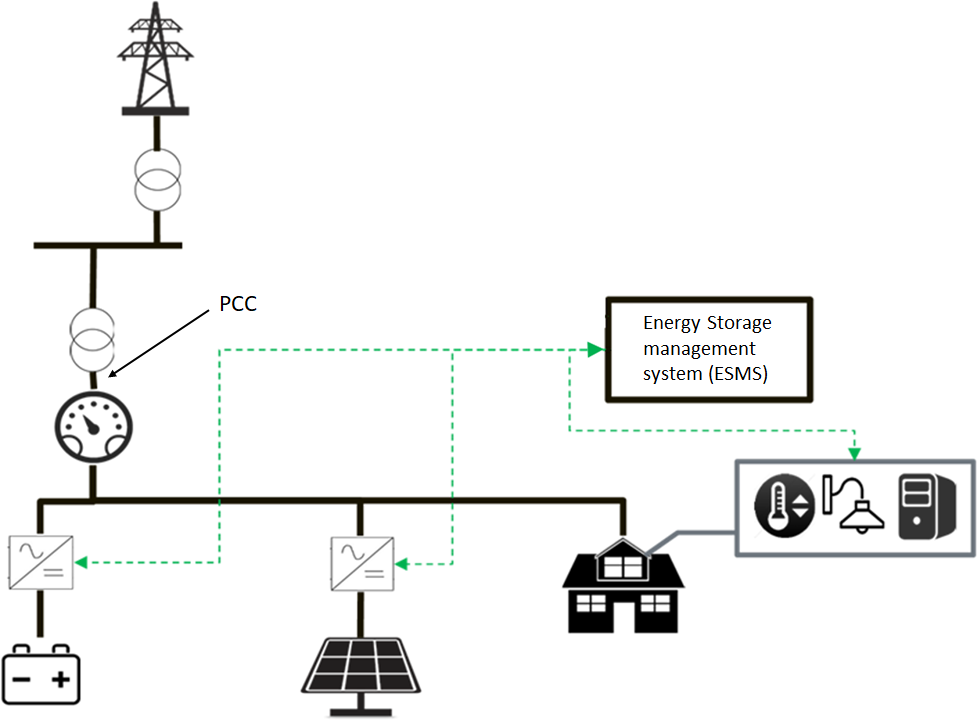
\includegraphics[width=\linewidth]{figs/System_architecture.png}
\caption{Test system architecture}
\label{fig:system_arch}
\vspace{-3mm}
\end{figure}

%  Fig. \ref{fig:F1_CA} shows the top-level architecture of the ESMS. As seen in the figure, the inputs of the system are the real-time price (RTP) prediction, load prediction, and the DG prediction, which in this case is a photovoltaic (PV) plant. It will also consider the current state of the load, PV generation, and ES. The output of the ESMS is the optimum battery charge and discharge control references based on the current and forecasted data.

\begin{figure}[!ht]
    \centering
    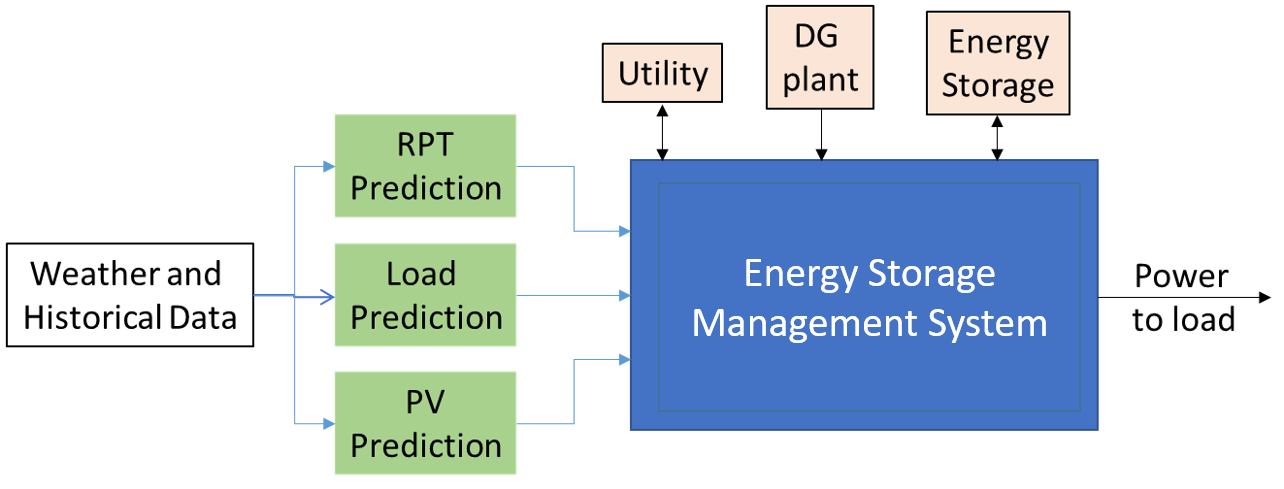
\includegraphics[width = \linewidth]{figs/EMS_FIG.png}
    \caption{Controller top level architecture}
    \label{fig:F1_CA}
\end{figure}

In order to find the optimum cost solution based on the current status of the system and future forecasts, the optimization problem is formulated using a graph search problem approach. To represent the solution space of the problem as a graph, the state of charge (SOC) of the ES, and both the prediction horizon and the control horizon are discretized. Fig. \ref{fig:F1_Dis} demonstrates an example of the discretized solution space.
\begin{figure}[!ht]
    \centering
    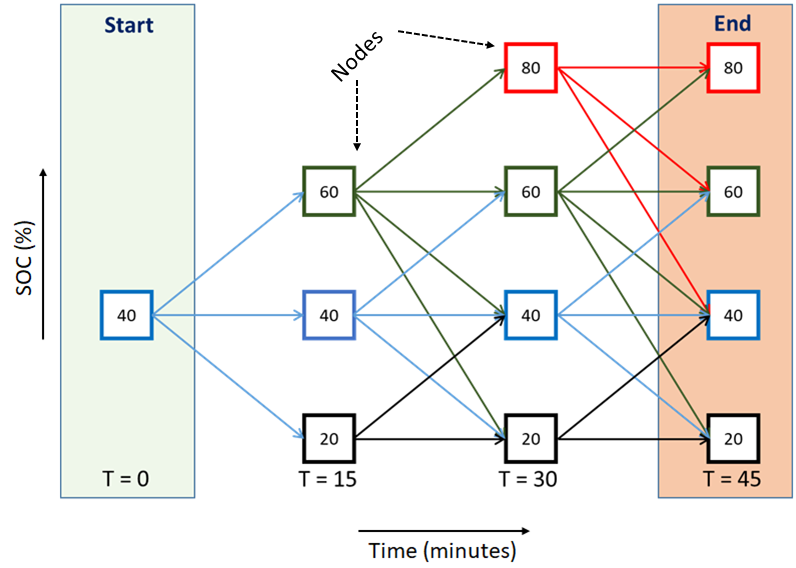
\includegraphics[width = \linewidth]{figs/F1_1_Dis.png}
    \caption{Discretizing solution space}
    \label{fig:F1_Dis}
\end{figure}
The horizontal axis of the figure represents time, and the vertical axis represents discrete steps in the state of charge (SOC) of the energy storage. In this simple example scenario, it is assumed that the algorithm recalculates the solution every 15 minutes (control horizon) based on available data. The SOC of the energy storage system (ESS) is discretized in steps of 20\%, and the SOC is limited between 80\% and 20\%. It is also assumed that the ESS can discharge a maximum of 40\% of its maximum SOC and charge a maximum of 20\% of its SOC in a 15 minute time step. These values are chosen arbitrarily in this simple example scenario to explain the problem. Taking these features into consideration, a directed graph is constructed looking ahead three time steps into the future. The square boxes represent nodes on the graph. The numbers inside the boxes represent the SOC of the ESS at that node. The arrows from the boxes represent all the possible states the ESS can be in the next time step according to the constraints of the system. The arrows are treated as edges of the graph. In this case, the edges are unidirectional. The goal is to find the most cost efficient path to reach T = 45 minute. Although in this example the algorithm considers T = 45 as the final stage, in actual application the final stage can be determined based on the actual use case.




\section{A* based energy management system} \label{A*}
By defining the solution space with a combination of nodes and edges the optimization problem can be formulated as a graph search problem. At the start the starting node is determined by the current status of the system. Then the following nodes and edges are generated using the forecasted data available. A discrete set of endpoints are set as the goals.The A*  algorithm runs for all the nodes and the node with the lowest path cost is selected as the best end node. The shortest graph search path to that node is selected as the optimum path.

The following are the main steps of the search algorithm,
\begin{enumerate}
\item \textbf{Set goal node:} Set the current goal node as the first component of the predefined list of end nodes. 
%2
\item \textbf{Create open list from start node:} Expand the start node and create an open list with all the child nodes of the start node. The open list sorts it's members in a priority queue based on the cost. The the start node is added to the closed list.
%3
\item \textbf{Select and expand best node from open list:} The node with the lowest cost is selected from the nodes within the open list. The Selected node is expanded and the children of the selected node is added to the open list. The expanded node is then added to the closed list.
%4
\item \textbf{Repeat 3 until goal node is reached}
%5
\item \textbf{Construct shortest path to goal node}: After reaching the goal node the shortest path to the goal is constructed from the closed list by retracing the parent nodes from the goal node to the start node.
%6
\item \textbf{Calculate and record total cost:} The total cost for the shortest path is calculated and the path is recorded with the total cost in a list named \textit{path list}.
%7
\item \textbf{Set new goal}: The open and closed list are cleared. The next component in the list of end nodes is selected as the goal node.
%8
\item \textbf{Repeat 2-7 for all components of the end nodes list}
%9
\item \textbf{Select the path with the lowest cost in the path list as the optimum path.}
\end{enumerate}

The EMS recalculates the optimum path using the search algorithm every time step based on the updated data of that time step. The system status is assumed to be unchanged between the time steps.

%\subsection{Cost Calculation}
The cost of going from a parent node to a child node is calculated by combining the real cost of getting to that child node and heuristic cost of getting to the goal from that child node. The real cost of going from a parent node $p$ at time $T=t$ to a child node $c$ at time $T=t+\Delta T$ is denoted as $C_{actual}(pc)$. It is calculated according to equation (\ref{eq:C_actual}).

\begin{equation}
\label{eq:C_actual}
    C_{actual}(pc) =  C_{ESS}(pc)+C_{GRID}(t)+C_{best}(p)
\end{equation}

Here, $\Delta T$ represents the time between two time steps. $C_{actual}(pc)$ represent the total cost of going to the child node $c$ from parent node $p$. $C_{ESS}(pc)$ represent cost of energy storage to go from parent node $p$ to child node $c$. $C_{GRID}(t)$ is the cost of using the grid between time $T=t$ and time $T=t+\Delta T$. $C_{best}(p)$ represent the best or least cost to get to node parent node $p$. $C_{ESS}(pc)$ is calculated according to equation \ref{eq:C_ESS}.

\begin{equation}
\label{eq:C_ESS}
C_{ESS}(pc) = |(SOC_p - SOC_c)|*ESS_{CAP}*R_{ESS} 
\end{equation}
Here, $SOC_p$ and $SOC_c$ represent the state of charge at parent and child node. $ESS_{CAP}$ represent the total energy capacity of the energy storage. And $R_{ESS}$ is the $\$/kWh$ cost of using the energy storage. $C_{GRID}(t)$ is calculated according to equation \ref{eq:C_GRID}.

\begin{equation}
\label{eq:C_GRID}
C_{GRID}(t) = 
\begin{cases}
   E_{GRID}(t)*RTP(t),& \text{if } E_{GRID}(t)\geq 0\\
    E_{GRID}(t)*SP(t),& \text{if }  E_{GRID}(t) < 0
\end{cases}
\end{equation}

Here, $E_{GRID}(t)$ is the energy drawn from the grid between time $T=t$ and time $T=t+\Delta T$. $RTP(t)$ is the real time price between $t$ and $t+\Delta T$. $SP(t)$ is the price the utility is willing to pay the consumer for selling power between $t$ and $t+\Delta T$.

The heuristic cost is calculated by assuming that whichever source has a smaller cost during a time step will supply the total demand of that time step. The heuristic cost of a node at time $T = t$ is calculated according to equation \ref{eq:C_H}.


\begin{equation}
\label{eq:C_H}
C_H(t) = \sum_{n=t}^{end} D(t)*R_{best}(t)
\end{equation}

Here, $C_H(t)$ represent the heuristic cost. $D(t)$ is the demand between time $T = t$ and time $T = t+\Delta T$. $R_{best}(t)$ is the source with the smaller cost which is calculated according to equation \ref{eq:R_best}

\begin{equation}
\label{eq:R_best}
R_{best}(t) = 
\begin{cases}
    R_{ESS},& \text{if } RTP(t)\geq R_{ESS}\\
    RTP(t),              & \text{otherwise}
\end{cases}
\end{equation}

After calculating the actual cost  $C_{actual}(pc)$ and heuristic cost $C_H(t)$ the total cost is calculated by adding  $C_{actual}(pc)$ and $C_H(t)$.



\section{Test system} \label{sys}
A microgrid similar to the one shown in Fig \ref{fig:system_arch} is constructed using the load and solar data collected form a Florida feeder available in the SUNGRIN project \cite{SUNGRIN} for testing the algorithm described in Section \ref{A*}. Table \ref{tab:solar_pv} shows the physical parameters of the PV plant and its inverter. The physical parameters of the energy storage used are shown in table \ref{tab:es}. The levelized cost of energy (LCOE)  of the energy storage system $R_{ESS}$ is calculated using equation \ref{eq:R_ESS}.

\begin{equation}
\label{eq:R_ESS}
R_{ESS} = \dfrac{ES_{tot}}{Cyc\cdot ES_{Cap}\cdot DoD\cdot \eta_{r}},
\end{equation}

%%%%%%%%PV%%%%%%%%%%%%%%%%%%%%%%%%%%%%%%%%%%%
\begin{table}[htb]
\normalsize
\renewcommand{\arraystretch}{1}
\caption{PV System Specifications}
\label{tab:solar_pv}
\centering
    \begin{tabular}{ | l | p{3cm} | }
    \hline
    \textbf{PV System Parameters} & \textbf{Value} \\ \hline
    PV Panels Rating (\(P_{PV}\)) & 875 kW  \\ \hline
    Inverter Rating (\(S_{PV}\)) & 900 kVA \\ \hline
    Power Factor Range (\(pf_{PV}\)) & 0.8-1.0  \\ \hline
    Max. Reactive Power (\(\overline{Q_{PV}}\)) & 540 kVAR \\ \hline
    Min. Reactive Power (\(\underline{Q_{PV}}\)) & -540 kVAR \\ \hline
    LCOE (\(r_{PV}\)) & 2.51 c/kWh \\ \hline
    \end{tabular}
    \begin{tabular}{l}
    \end{tabular}
\end{table}
%%%%%%%%PV%%%%%%%%%%%%%%%%%%%%%%%%%%%%%%%%%%%


%%%%%%%%ES%%%%%%%%%%%%%%%%%%%%%%%%%%%%%%%%%%%
\begin{table}[htb]
\normalsize
\renewcommand{\arraystretch}{1}
\caption{Energy Storage (ES) System Specifications}
\label{tab:es}
\centering
    \begin{tabular}{ | l | p{3cm} | p{3cm} | }
    \hline
    \textbf{ES System Parameters} & \textbf{Value} \\ \hline
    ES Rating (\(P_{ES}\)) & 750 kW  \\ \hline
    Inverter Rating (\(S_{ES}\)) & 750 kVA \\ \hline
    Max. State of Charge  (\(\overline{SOC_{ES}}\)) & 2190 kWh \\ \hline
    Min. State of Charge  (\(\underline{SOC_{ES}}\)) & 219 kWh \\ \hline
    Power Factor Range (\(pf_{ES}\)) & 0.8-1.0  \\ \hline
    Max. Reactive Power (\(\overline{Q_{ES}}\)) & 450 kVAR \\ \hline
    Min. Reactive Power (\(\underline{Q_{ES}}\)) & -450 kVAR \\ \hline
    LCOE (\(r_{ES}\)) & 12.3 c/kWh \\ \hline
    \end{tabular}
\end{table}
%%%%%%%%ES%%%%%%%%%%%%%%%%%%%%%%%%%%%%%%%%%%%

The load and solar profile for the testing of the algorithm were obtained from the SUNGRIN project. Fig \ref{fig:LOAD_PROFILE_8} shows the load profile of the system for eight days with average, minimum and maximum loads.

\begin{figure}[!ht]
    \centering
    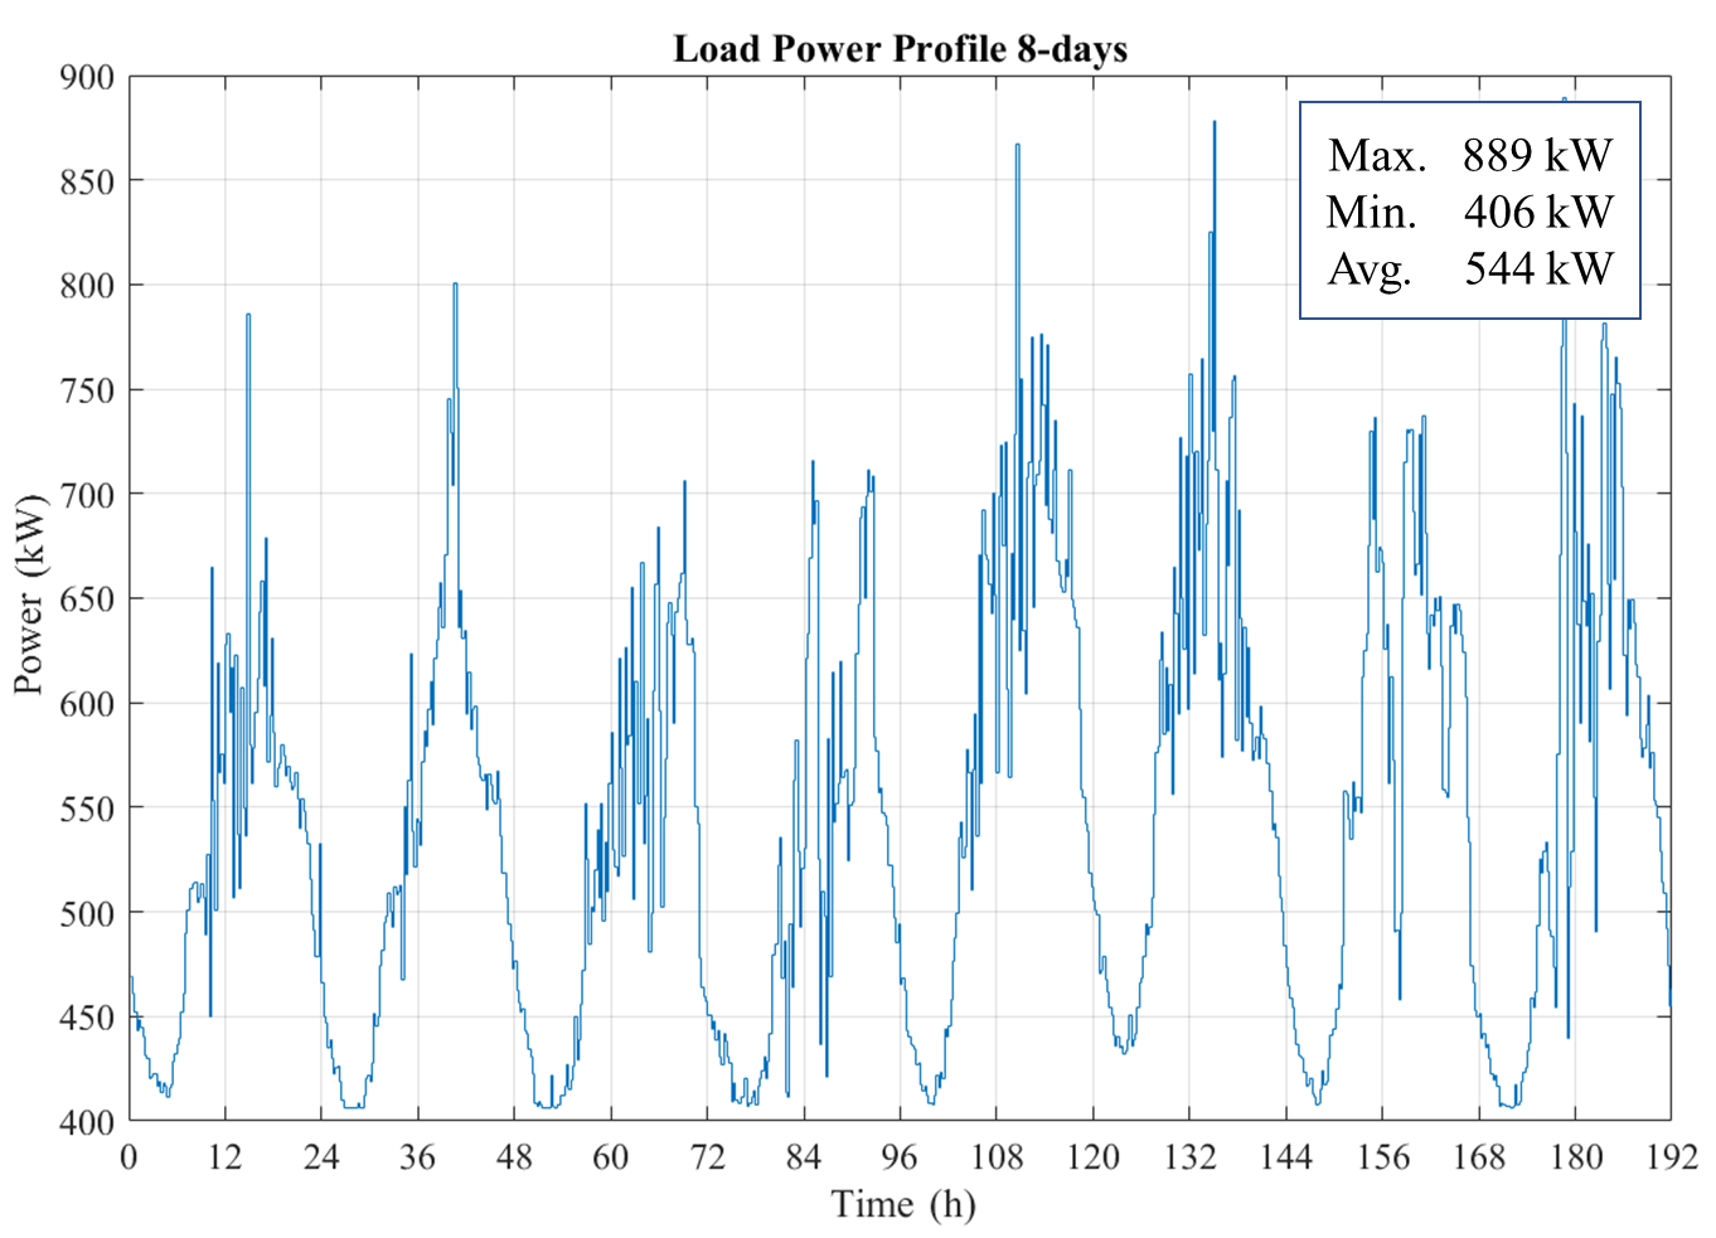
\includegraphics[width = \linewidth]{figs/loadprofile.png}
    \caption{Eight day load profile}
    \label{fig:LOAD_PROFILE_8}
\end{figure}

To generate the RTP profile Locational Based Marginal Pricing (LBMP) data is collected from the New York Independent System Operator (NYISO) \cite{NYISO2017}. The collected LBMPO is combined with the time of use price available at Tallahassee to generate a RTP for the test case. Fig \ref{fig:RTP_PROFILE_8} shows the real-time price profile used for the test system. The system is also tested against time of use pricing scheme available from PG\&E \cite{pgne}. Fig \ref{fig:PGNE_PRICE} shows the price profile acquired from PG\&E.

\begin{figure}[!ht]
    \centering
    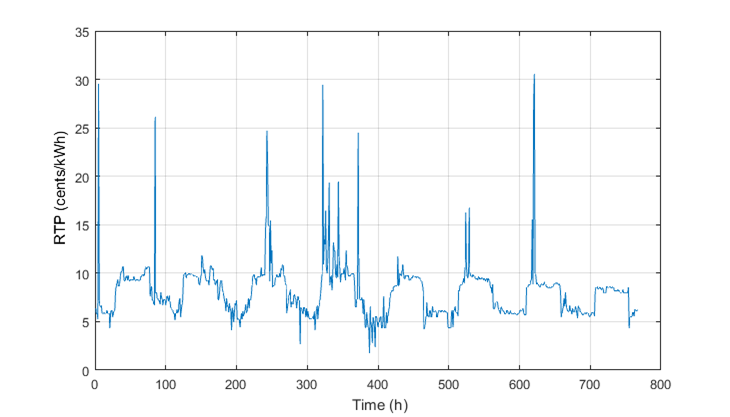
\includegraphics[width = \linewidth]{figs/rtp_8days.png}
    \caption{Eight day RTP profile NYISO}
    \label{fig:RTP_PROFILE_8}
\end{figure}

\begin{figure}[!ht]
    \centering
    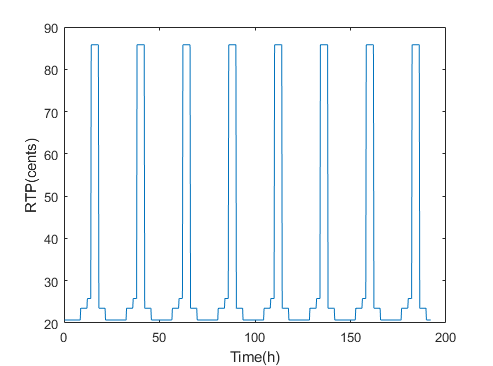
\includegraphics[width = \linewidth]{figs/PGNE_PRICE.png}
    \caption{Eight day RTP profile PG\&E}
    \label{fig:PGNE_PRICE}
\end{figure}

The PV profile used in the system is collected from the SUNGRIN project and scaled to fit the ratings of the PV described in table \ref{tab:solar_pv}. Fig \ref{fig:PV_PROFILE_8} shows the eight-day PV profile used.

\begin{figure}[!ht]
    \centering
    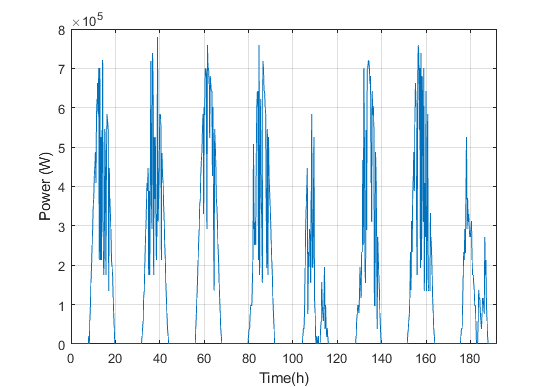
\includegraphics[width = \linewidth]{figs/PV_PROFILE.png}
    \caption{Eight day PV profile}
    \label{fig:PV_PROFILE_8}
\end{figure}

\section{Offline simulation and results} \label{OFF}
The system described in Section \ref{sys} is modeled and simulated in MATLAB\textsuperscript{\textregistered} Simulink\textsuperscript{\textregistered} using the Simscape Power Systems\textsuperscript{TM} toolbox. The A* based ESM is run using the described data, and the results are fed in as an open loop control to a Simulink model for phasor simulation. In the test cases, the energy management problem is formulated according to the formulation discussed in Section \ref{formulation}. The  SOC of the ESS is discretized in steps of 2\%, and the SOC is limited between  94\%  and  10\%. The time step and the control horizon chosen is 15 minutes. The ES is allowed to charge or discharge a maximum of 8\% of its total capacity during one time-step. The 8\% limitation is set based on the power specifications discussed in table \ref{tab:es}. The A* search runs every 15 minutes considering a 24 hours (96 time-steps) prediction horizon. The performance of the A* based ESM is compared against two sample base test cases. The base test cases are the following:

\begin{enumerate}
\item \textbf{Case 1:} Charging the ES from 2 AM to 5 AM, Discharging the ES from 7 PM to 11 PM

\item \textbf{Case 2:} Charging from the ES 11 AM to 2 PM, Discharging the ES from 7 PM to 11 PM
\end{enumerate}

All the test cases are run under two different scenarios. Net metering scheme and different selling-buying energy price.

\subsection{Comparison considering net metering} \label{netmeter}
In this scenario, the A* based EMS is compared against the two base test cases considering net metering. The NYISO RTP scheme shown in Fig. \ref{fig:RTP_PROFILE_8} is used for this comparison. The price of the energy storage is chosen as 12.6 \cent/kWh. This price is calculated based on the specifications of the Tesla Powerpack \cite{tesla_powerpack_2018}.


Fig. \ref{fig:SBMPO_COMP_1_day} shows a zoomed view of the first day of the 7-day simulation for the A* based EMS. The solid black line in the figure represents the SOC of the energy storage, and the dotted red line represents the RTP. The dashed blue line represents the Demand. The left vertical axis of the graph represents the RTP of energy and the SOC of the ES. The right vertical axis represents the kWh demand of the system. A negative demand represents excess energy from the local generation after fulfilling the local demand. The horizontal axis represents time in 15-minute time steps. The arrows with the numbers showing specific points of the figure that are explained next, based on the behavior of the EMS. As observed in Fig. \ref{fig:SBMPO_COMP_1_day}, there are two peaks in price at the points 1 and 3 throughout the 24 hours (96-time step) window of operation.  The ESM accurately anticipates the price peak in point 1 and charges the energy storage using the grid just before the peak occurs, and discharges during the price peak at point 1. It can be seen that during the peak, the demand was positive and the cheapest available price for grid energy was available just before the peak. The algorithm also anticipates the next price peak at point 3 based on forecasted data and prepares the ES to discharge at that price peak by charging at the lowest RTP period at point 2. Although, there is an excess generation available from the PV in between point 2 and point 3 the opportunity cost of using the PV to charge the ES will be equal to the RTP due to net metering. So, in this case, the algorithm behaves as expected and uses the lowest possible RTP period to charge the ES and discharges during the price period when there is a high enough price peak to justify the use of the energy storage.

\begin{figure}[!ht]
    \centering
    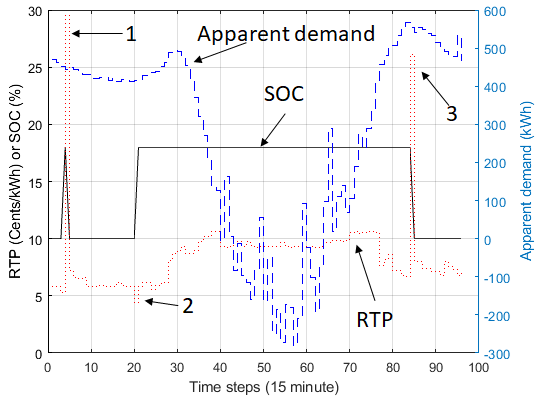
\includegraphics[width = \linewidth]{figs/SBMPO_COMP_1_day.png}
    \caption{First day EMS response for net metering comparison case}
    \label{fig:SBMPO_COMP_1_day}
\end{figure}

Fig. \ref{fig:SBMPO_COMP_10_12} shows the response of the A*-based EMS in a  7 days run used in the same microgrid system.  It can be seen from the figure that the A*-based ESM is following the same behavior displayed in Fig. \ref{fig:SBMPO_COMP_1_day}. It's taking advantage of the lowest energy price before a price peak appears in its prediction horizon, and charging the energy storage in order to discharge it when there is a high enough price peak. The total cost of operation for the A*-based ESM for the 7 day period is shown in Table \ref{tab:Cost1}

\begin{table}[htb]
\caption{Seven day Cost for the three cases (net metering)}
\label{tab:Cost1}
\begin{tabular}{|l|l|}
\hline
Case1 & \$7,086 \\ \hline
Case2 & \$8,601 \\ \hline
A* Case & \$4,861 \\ \hline
A* Case \% savings (Case1) & 31.40\% \\ \hline
A* Case \% savings (Case2) & 43.48\% \\ \hline

\end{tabular}
\end{table}


\begin{figure}[!ht]
    \centering
    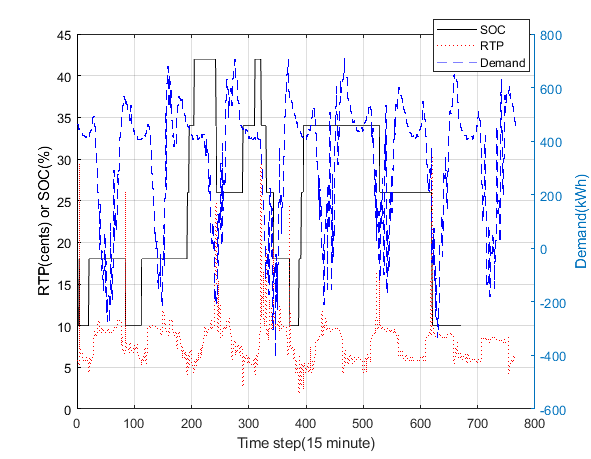
\includegraphics[width = \linewidth]{figs/SBMPO_COMP_10_12.png}
    \caption{Full 7 day EMS response for net metering comparison case}
    \label{fig:SBMPO_COMP_10_12}
\end{figure}


\subsection{Test result considering different buying and selling price of energy}
In this scenario, the proposed algorithm is tested against the two base test cases using different price for selling power back to the grid. The cases 1 and 2 are previously fixesd standard control strategies based on predefined charging and discharging of the energy storage mentioned before. A* based ESM control is implemented with a control horizon of 15 minutes and a prediction horizon of 24-hours. For these test cases, it is assumed the energy storage starts at the lower bound of SOC (10 \%).

Fig. \ref{fig:VAR_1_day_example} shows the 1 day test result for the A*-based EMS considering the RTP scheme shown in Fig. \ref{fig:RTP_PROFILE_8} for buying power and considering a sell-back price of 4 cents/kWh. The other system parameters are kept the same as the system used in the previous scenario. As seen in Fig. \ref{fig:VAR_1_day_example}, there are two peaks in price at the points 1 and 3 throughout the 24 hours (96-time step) window of operation. The ESM properly anticipates charges the energy storage using the grid just before the peak occurs and discharges during the price peak at point 1, similar to the behavior observed in the previous scenario. The next price peak is at point 3, and the lowest price for grid power available for charging the storage is at point 4. In case of a net metering scheme, point 4 would have been the best time to charge the ES in order to discharge it during the next price peak. But due to the fact that a sell-back price of 4 cents/kWh is being considered, this is no longer the case. The price 4 cents/kWh is lower than the price of buying grid energy at point 4. So the A*-based EMS takes into account the lowest opportunity cost of selling power back to the grid and decides to charge the ES during point 2 when there is additional local generation available. This behavior demonstrates that the A*-based ESM can use the forecasted knowledge of the future demand and RTP together to automatically decide the best moments to operate the energy storage depending on different pricing schemes.

 \begin{figure}[!ht]
    \centering
    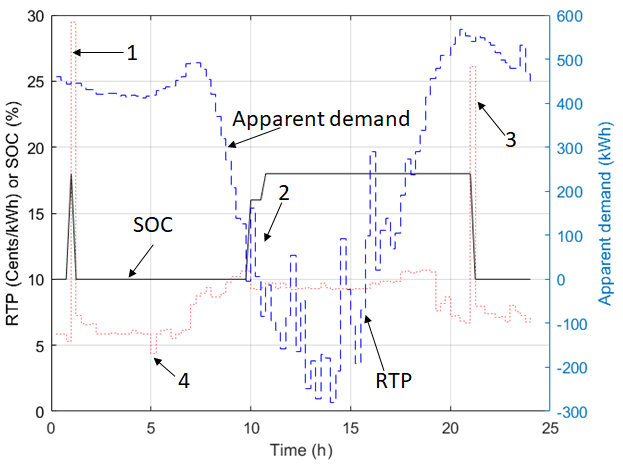
\includegraphics[width = \linewidth]{figs/VAR_1_day_example.png}
    \caption{1 day EMS response considering NYISO price and 4 centes/kWh sellback price}
    \label{fig:VAR_1_day_example}
\end{figure}

Fig. \ref{fig:VAR_10_12_4} shows the 7-day test result for the tested microgrid considering the RTP shown in Fig. \ref{fig:RTP_PROFILE_8} and a sell-back price of 4 cents/kWh. Fig. \ref{fig:VAR_10_12_30rtp} shows the 7-day test results for the same RTP considering a sell-back price of 30\% of the RTP. Fig. \ref{fig:PG_VAR_10_12_4} and Fig. \ref{fig:PG_VAR_10_12_30rtp} show the ESM operation for the PG\&E profile shown in Fig. \ref{fig:RTP_PROFILE_8} considering 4 cents/kWh and 30\% of the RTP sell-back price respectively. It can be observed from the 7-day cases, that the A*-based ESM shows behavior similar to the behavior seen in  Fig. \ref{fig:VAR_1_day_example}. The costs for the different conditions considered in the three cases are shown in Table \ref{tab:Cost}. Depending on the test case evaluated, the A* based ESM shows substantial cost savings of around 6.93\% to 41.79\%. 

 \begin{figure}[!ht]
    \centering
    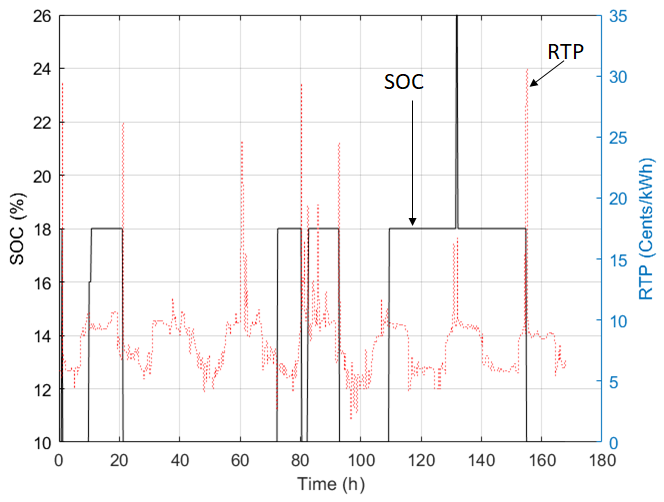
\includegraphics[width = \linewidth]{figs/VAR_10_12_4.png}
    \caption{7 day EMS response considering NYISO price and 4 centes/kWh sell back price}
    \label{fig:VAR_10_12_4}
\end{figure}

 \begin{figure}[!ht]
    \centering
    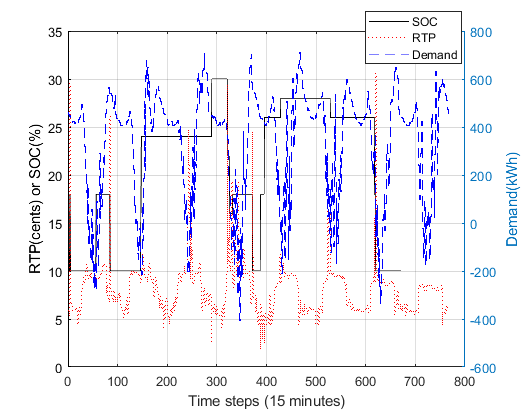
\includegraphics[width = \linewidth]{figs/VAR_10_12_30rtp.png}
    \caption{7 day EMS response considering NYISO price and 30\% of RTP sell back price}
    \label{fig:VAR_10_12_30rtp}
\end{figure}

 \begin{figure}[!ht]
    \centering
    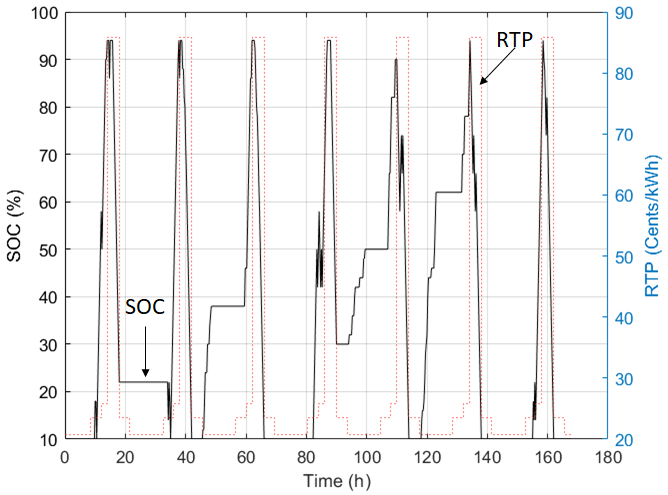
\includegraphics[width = \linewidth]{figs/PG_VAR_10_12_4.png}
    \caption{7 day EMS response considering PG\&E price and 4 centes/kWh sell back price}
    \label{fig:PG_VAR_10_12_4}
\end{figure}

 \begin{figure}[!ht]
    \centering
    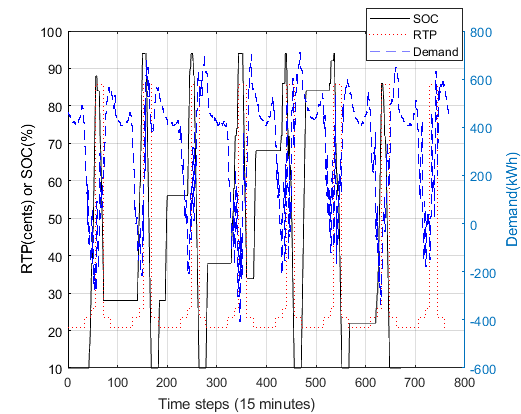
\includegraphics[width = \linewidth]{figs/PG_VAR_10_12_30rtp.png}
    \caption{7 day EMS response considering PG\&E price and 30\% of RTP sell back price}
    \label{fig:PG_VAR_10_12_30rtp}
\end{figure}


%%%%%%%%CSOT%%%%%%%%%%%%%%%%%%%%%%%%%%%%%%%%%%%
\begin{table}[htb]
%\normalsize
%\renewcommand{\arraystretch}{1}
\caption{Seven day Cost for the three cases (different sell price)}
\label{tab:Cost}
\centering

\begin{tabular}{l|l|l|l|l|}
\cline{2-5}
                            & \multicolumn{2}{l|}{4 cents/kWh} & \multicolumn{2}{l|}{30\% RTP}   \\ \cline{2-5} 
                            & NYISO           & PG\&E          & NYISO          & PG\&E          \\ \hline
\multicolumn{1}{|l|}{Case1 cost} & \$8,265  & \$19,396 & \$8,314 & \$19,109 \\ \hline
\multicolumn{1}{|l|}{Case2 cost} & \$8,8606  & \$19,633 & \$8,895 & \$19,407 \\ \hline
\multicolumn{1}{|l|}{A* Case cost} & \$5,329  & \$18,051 & \$5,178 & \$17,106 \\ \hline
\multicolumn{1}{|l|}{A* Case \% savings (Case1)} & 35.52\%         & 6.93\%         & 37.72\%        & 10.84\%        \\ \hline
\multicolumn{1}{|l|}{A* Case \% savings (Case2)} & 39.85\%         & 8.08\%         & 41.79\%        & 11.86\%        \\ \hline
\end{tabular}

\end{table}
%%%%%%%%CSOT%%%%%%%%%%%%%%%%%%%%%%%%%%%%%%%%%%%




%%%%%%%%COMPARE_COST%%%%%%%%%%%%%%%%%%%%%%%%%%%%%%%%%%%
% \begin{table}[htb]
% %\normalsize
% %\renewcommand{\arraystretch}{1}
% \caption{Case 3 savings compared to other cases (7 days)}
% \label{tab:Cost_comp}
% \centering
% \begin{tabular}{l|l|l|l|l|}
% \cline{2-5}
%                             & \multicolumn{2}{l|}{4 cents/kWh} & \multicolumn{2}{l|}{30\% RTP}   \\ \cline{2-5} 
%                             & NYISO           & PG\&E          & NYISO          & PG\&E          \\ \hline
% \multicolumn{1}{|l|}{Case1} & 35.52\%         & 6.93\%         & 37.72\%        & 10.84\%        \\ \hline
% \multicolumn{1}{|l|}{Case2} & 39.85\%         & 8.08\%         & 41.79\%        & 11.86\%        \\ \hline
% \end{tabular}
% \end{table}
% %%%%%%%%COMPARE_COST%%%%%%%%%%%%%%%%%%%%%%%%%%%%%%%%%%%

\section{Real-time simulation and results} \label{RT}
A controller hardware in the loop (CHIL) simulation was set up to validate the algorithm in a real-time environment. 
The block layout of the CHIL simulation is shown in Fig. \ref{fig:RT_block}. The power system shown in Fig. \ref{fig:simulation_grid}, is simulated in real time in a digital real-time simulator (DRTS) with a time step of 50 ${\mu}s$. This system is modeled for detailed electromagnetic transient simulation unlike the phasor simulation model used in the offline simulation. The A* based ESM algorithm is implemented in Python 2.7 on a windows machine. The specifications of the machine are given in Table \ref{tab:PC}. The communication link between the DRTS and windows machine was established using TCP/IP. The DRTS sent the windows machine running the ESM the current PV generation ($P_{PV}(t)$), the current load ($P_load(t)$) and the current energy storage state of charge ($ES_{SOC}(t)$). The RTP, Load and PV prediction profiles are fed to the ESM by a pregenerated MATLAB formatted data (MAT) file. The current RTP is also provided by the MAT file. After receiving the current status and predicted profiles the ESM determines the power the ES should provide for the current time period ($P_{ES}(t)$) and sends it back to the DRTS. The actual CHIL setup is shown in Fig. \ref{fig:LAB_REAL}. 

\begin{table}[htb]
\caption{Windows machine specification}
\label{tab:PC}
\centering
\begin{tabular}{|l|l|}
\hline
Operating system & Windows 10 Home 64-bit      \\ \hline
Processor        & Intel(R) Core(TM) i5-7300HQ \\ \hline
Memory           & 8192 MB RAM                 \\ \hline
\end{tabular}
\end{table}

\begin{figure}[!ht]
    \centering
    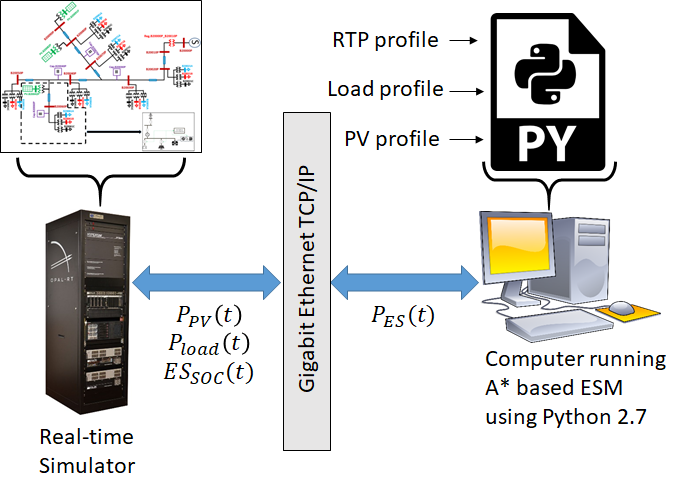
\includegraphics[width = \linewidth]{figs/RT_block.png}
    \caption{Block layout of the CHIL setup}
    \label{fig:RT_block}
\end{figure}




\begin{figure}[!ht]
    \centering
    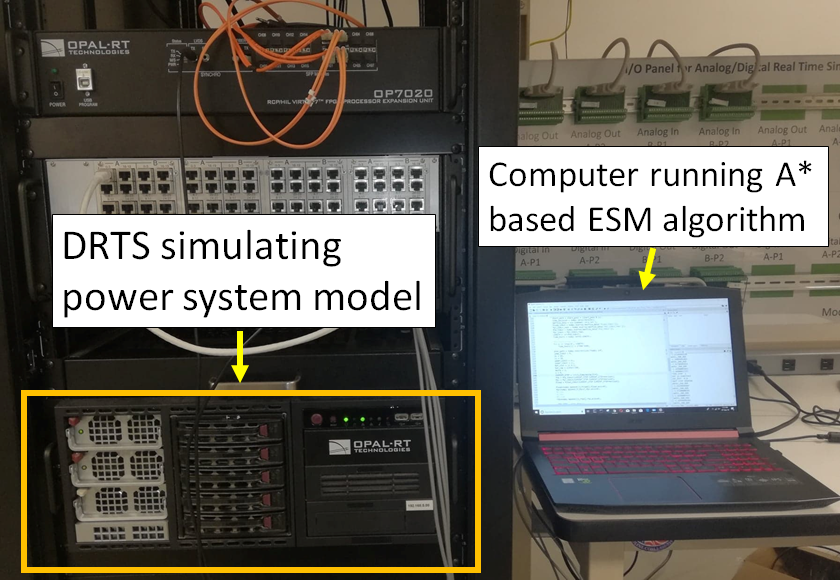
\includegraphics[width = \linewidth]{figs/LAB_REAL.png}
    \caption{Actual CHIL setup}
    \label{fig:LAB_REAL}
\end{figure}

For the CHIL simulation, the ESM algorithm was set up according to the setup described in Section \ref{OFF}. The  SOC of the ESS is discretized in steps of 2\%, and the SOC is limited between  94\%  and  10\%. The time step and the control horizon chosen is 15 minutes. The ES is allowed to charge or discharge a maximum of 8\% of its total capacity during one time-step. The A* search runs every 15 minutes considering a 24 hours (96 time-steps) prediction horizon. The price profile used was the NYISO price profile. The net metering scenario was considered. The cost of the ES was kept 12.3 cents/kWh. The simulation was run for 50 hours (200 time steps) in real-time. Fig. \ref{fig:RT_TESTING} shows the real-time and the offline simulation results for the 50 hour run. It can be seen that the real-time simulation result shown by the dotted lines follows the off-line simulation result shown by the solid line. The results are similar to the first two days of Fig. \ref{fig:SBMPO_COMP_10_12} as expected. The comparison of the real-time and offline cost savings of the algorithm is shown in table \ref{tab:rt_cost}. It can be seen from the table that the real-time cost savings is comparable to the offline results.



\begin{figure}[!ht]
    \centering
    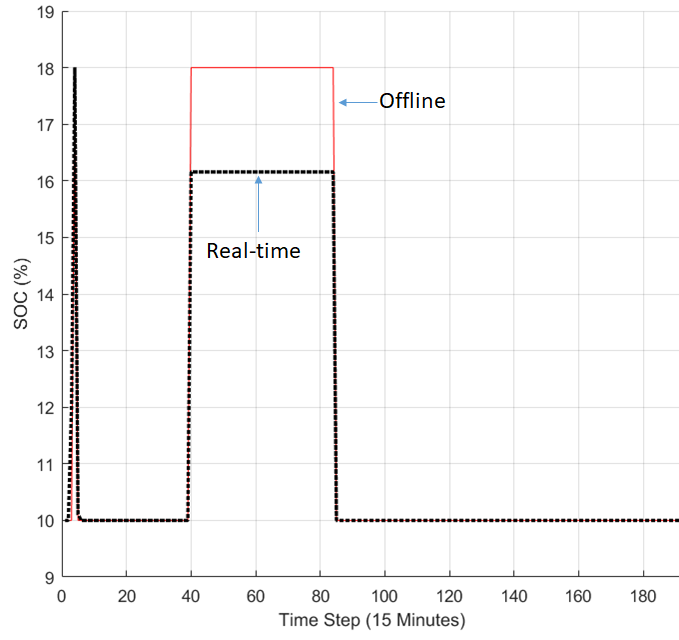
\includegraphics[width = \linewidth]{figs/RT_TESTING.png}
    \caption{Real-time vs offline result (50  hours)}
    \label{fig:RT_TESTING}
\end{figure}



\begin{table}[htb]
\centering
\caption{Real-time simulation cost (48 hours)}
\label{tab:rt_cost}
\begin{tabular}{l|l|l|l|}
\cline{2-4}
                                          & Real-time & Offline & Difference \\ \hline
\multicolumn{1}{|l|}{Case1}               & \$1,662   & \$1,579 & 4.99\%     \\ \hline
\multicolumn{1}{|l|}{Cas2}                & \$1,713   & \$1,628 & 4.96\%     \\ \hline
\multicolumn{1}{|l|}{A* Case}             & \$1,345   & \$1,286 & 4.39\%     \\ \hline
\multicolumn{1}{|l|}{A* savings (Case 1)} & 19.07\%   & 18.56\% & 0.52\%     \\ \hline
\multicolumn{1}{|l|}{A* savings (Case 2)} & 21.48\%   & 21.01\% & 0.48\%     \\ \hline
\end{tabular}
\end{table}

\section{Novelty of research} \label{Novelty}
The novelty of the research is as follows
\begin{itemize}
    \item Implemented a real-time ESM algorithm capable of considering the future as well as present status of the system.
    \item The algorithm finishes computation relatively quickly. It responded within two seconds in the CHIL testing while using the relatively inexpensive hardware specifications shown in table \ref{tab:PC}.
    \item The algorithm is capable of considering different pricing schemes.
    \item The algorithm is easily scalable. The discretization and prediction horizon can be easily scaled to incorporate various needs.
    \item The algorithm is designed in python 2.7 making it easily deployable in a variety of hardware without the need of any proprietary software.
\end{itemize}

\section{Conclusions}
This paper proposed a novel ESM aimed to determine the optimal cost of ES. The ESM scheme is designed to optimize the charging and discharging of grid-connected energy storage by formulating the problem as a graph search and solving the graph search using the A* search algorithm. The A* based ESM is tested using real data collected from the SUNGRIN project, NYISO, and PG\&E. It also considers both a net metering scenario and a different sell back price scenario where the buying price of energy is different from the selling price. The ESM shows a cost saving of 6.93\% to 43.48\% compared to the base test cases for the tested scenarios. The results show that the proposed method has the capability to adapt to various varying price profiles and system status and provides a solution that reduces cost significantly. Future research will focus on developing an ESM capable of controlling multiple ES and additional DERs taking into account system constraints.

\bibliographystyle{IEEEtran}
\bibliography{mybib.bib}

\ifCLASSOPTIONcaptionsoff
  \newpage
\fi

\end{document}
